\section{实验过程与结果}
\subsection{自采集数据呈现}

\subsubsection{摄像头分布与分组}

\subsubsection{打好标签的数据集}

\subsection{行人重识别算法}

\subsubsection{训练Loss曲线}

\subsubsection{测试准确率比较}

\subsubsection{测试结果可视化}

\subsection{强化学习算法}

\subsubsection{学习后选择的部署方案}

\subsection{分布式CPU训练}

\subsubsection{与单机的比较}

\subsubsection{与GPU的比较}

\subsection{实验过程}
实验环境为天河二号的GPU分区,一共使用了4个节点,每个节点配有NVIDIA Tesla K80显卡,
显卡的RAM为11GB,支持单机多卡运算。

将写好的代码传入天河二号中转机,然后为每个节点创建作业进程,每个进程除了rank不一致外,
其它部分都相同。

创建作业之后可以使用yhq命令查看当前作业队列的执行情况。如下图所示。从图中可以看到当前
一共有5个作业正在执行,执行的分区是天河二号的GPU分区,作业的脚本名称为reid.sh,当前的
状态是R,代表着正在运行,作业已经正常运行了24分钟38秒,每个作业占用了1个节点,节点的
名称分别是gn10 - gn14。\\[0.5cm]
\includegraphics[width=1\textwidth]{figure/yhq}

使用SSH登录计算节点后,可以用top命令查看CPU的占用情况。如下图所示。从图中可以看出
python进程只占用了CPU的10个核心,主要用于训练数据的搬运和预处理,以及各节点之间的通信。
由于训练数据集采用了边用边读的方式,所以内存占用很少。\\[0.5cm]
\includegraphics[width=1\textwidth]{figure/top}

使用nvidia-smi命令可以查看GPU的占用情况。如下图所示。可以看到gn10节点有4块NVIDIA Tesla K80
显卡,每一张的显存是11GB,模型的训练进程将4张卡都占用了,正在并行地计算。\\[0.5cm]
\includegraphics[width=1\textwidth]{figure/smi}
\subsection{实验结果}
\subsubsection{训练}
图\ref{fig:loss}为训练过程的交叉熵误差随着迭代次数的变化曲线:

图例64-5-60表示训练的Batch Size是64,分布式训练的节点数为5,Epoch数为64。需要注意的是,
图中不同节点数的曲线,其训练完成所花费的时间是不一样的,2个节点的训练过程大约需要11个小时,
1个节点的训练大约需要22个小时。从图中可以看到在相同的迭代次数下,节点数越少,误差下降得越快。

其中的原因是,并行训练的原理是将训练数据随机分块并分配给各节点,各节点用该部分数据独立地进行
Forward和Backward操作,计算梯度,最后与其它节点共享梯度,完成参数更新。只使用部分的数据,
计算出来的梯度方向不会比用全部数据计算出来的更准确。虽然大体上梯度下降的方向是没错的,但是使用
分布式训练明显走了很多“弯路”,并且节点数越多,下降的相对速度就越慢。
\begin{figure}
\centering
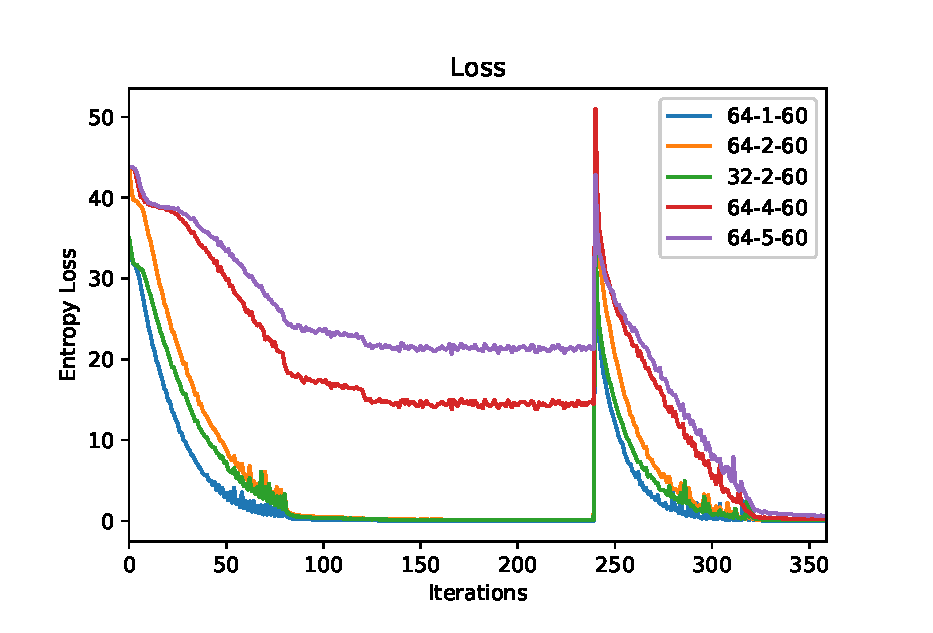
\includegraphics[width=1\textwidth]{figure/loss}
\caption{交叉熵误差随着迭代次数变化曲线}
\label{fig:loss}
\end{figure}
但是在绝对速度的比较上,训练过程所需的绝对时间还是与节点数成反比的,毕竟有更多的节点来分担
计算任务。例如单机训练需要花费22个小时,采用5个节点分布式训练只需要花费5个小时左右。

以上是采用单机训练和多机分布式训练的差异。对于最终训练结果,不管采用单机还是分布式,都会收敛到
一个相近的误差,即虽然过程有差异,但结果差异不大。证明了分布式训练是一种可行的加快训练速度的
方法。

\subsubsection{测试}
表\ref{tab:test}为在Market1501测试集上的测试结果:
\begin{table}[]
\centering
\caption{Market1501测试结果}
\label{tab:test}
\begin{tabular}{@{}lllll@{}}
\toprule
        & Rank1 & Rank5 & Rank10 & mAP  \\ \midrule
64-1-60 & 91.4  & 97.1  & 98.1   & 77.2 \\
64-2-60 & 89.6  & 96.3  & 97.8   & 75.2 \\
32-2-60 & 90.5  & 96.7  & 98.0   & 76.8 \\
64-4-60 & 89.5  & 96.1  & 96.7   & 75.4 \\
64-5-60 & 89.9  & 96.3  & 97.2   & 75.6 \\ \bottomrule
\end{tabular}
\end{table}

可以看出分布式训练结果的精度在误差允许的范围内。
